%! suppress = UnresolvedReference
% \usepackage{amsfonts}
% \usepackage{amsmath}
% \usepackage{graphicx}
% \usepackage{mathtools}

\subsection{Arithmetic expression}\label{sec:expression}

In order to define arithmetic expressions involving real numbers  $\mathbb{R}$ in a rigorous way, we need to use a sophisticated type theory.
However, in order to keep things simple and maintain clarity, we will start by using only production rules, but with certain semantic restrictions.
We will also begin with rational numbers $\mathbb{Q}$ to avoid the difficulties inside real numbers $\mathbb{R}$ .

\begin{definition}\label{def:arithmetic-expression}
    An arithmetic expression $a$ over $\mathbb{Q}$ is a structure given by the following production rules:
\begin{equation}\label{eq:productionrule}
\begin{aligned}
a &\longleftarrow x\\
a &\longleftarrow ( a + a )\\
a &\longleftarrow ( a - a )\\
a &\longleftarrow ( a \times a )\\
a &\longleftarrow ( a \div a )
\end{aligned}
\end{equation}
    where $x \in \mathbb{Q}$, and we denote this as $a \in \mathbb{E} \left [\mathbb{Q} \right ]$.
\end{definition}

During the production process, we can obtain both a string representation and a tree representation of arithmetic expression $a$,
where the two representations are equivalent.
For instance, the string representation of $a$ might be:

\begin{equation}
(((((1 \times 2) \times 2) - 1) \times (2 + 1)) - 6)\label{eq:equation}
\end{equation}

and the parsed syntax tree is depicted in Figure~\ref{fig:syntaxtree}.

\begin{figure}[ht]
\centering
\resizebox{0.2\textheight}{!}{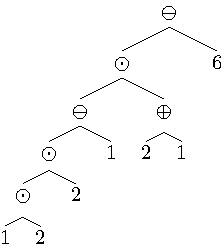
\includegraphics{images/02-example-expression-syntax-tree.pdf}}
\caption{a tree representation of an arithmetic expression}\label{fig:syntaxtree}\label{fig:figure}
\end{figure}

If we interpret the target as a string and the building processes in production rule~\eqref{eq:productionrule} as string building, we get the \emph{string representation}.
On the other hand, if the target is a tree, tree building leads to the \emph{tree representation}.
We can easily obtain the string representation of $a$ from its tree representation by performing a pre-order traversal.

The concept of a \emph{sub-expression} can also be derived from the concept of a subtree.
The branch nodes are all labeled with operators: $+$, $-$, $\times$, $\div$.
The leaf nodes are all labeled with numbers.

Evaluation $\nu$ is a partial function that operates on arithmetic expression $a \in \mathbb{E} \left [\mathbb{Q} \right ]$.
It is undefined only if division by zero occurs during the recursive evaluation process.

We can define evaluation $\nu(a)$ of $a$ recursively as follows:
\begin{itemize}
  \item Constant leaf: for any $x \in \mathbb{Q}$, $\nu(x) = x$.
  \item Compositional node by $+$: For any $(a + b)$, $\nu((a + b)) = \nu(a) + \nu(b)$.
  \item Compositional node by $-$: For any $(a - b)$, $\nu((a - b)) = \nu(a) - \nu(b)$.
  \item Compositional node by $\times$: For any $(a \times b)$, $\nu((a \times b)) = \nu(a) \nu(b)$.
  \item Compositional node by $\div$: For any $(a \div b)$, if $\nu(b) \neq 0$, then $\nu((a \div b)) = \nu(a) / \nu(b)$.
\end{itemize}

We say that an arithmetic expression $a$ is \emph{evaluable} if $\nu(a)$ is defined.
In the rest of this article, we will only consider evaluable arithmetic expressions unless stated otherwise.

Given an arithmetic expression $a$, whatever evaluable or not, we can obtain its tree representation.
If a node $l$ is a leaf node, its corresponding subexpression $s$ is a number, so we consider it to be already \("\)evaluated\("\).
If a node $b$ is a branch node, its corresponding subexpression $s$ is an expression, and we can apply $\nu$ to it to obtain a number $\nu(s)$.
During the recursive evaluation process, starting from the leaves and moving towards the root, the subexpressions are evaluated one after another.
However, the order of evaluations is generally not unique.

\begin{definition}
The evaluation order of an arithmetic expression $a$ is an ordering of branch nodes in the tree representation of $a$
such that every node (sub-expression) is evaluated before its parent.
\end{definition}

For example, the possible evaluation orders of the arithmetic expression in Figure~\ref{fig:syntaxtree} are:
\begin{itemize}
  \item $1 \times 2 \rightarrow \underline{2}; \underline{2} \times 2 \rightarrow \underline{4}; \underline{4} - 1 \rightarrow \underline{3}; 2 + 1 \rightarrow \underline{3}; \underline{3} \times \underline{3} \rightarrow \underline{9}; \underline{9} - 6 \rightarrow 3$
  \item $1 \times 2 \rightarrow \underline{2}; \underline{2} \times 2 \rightarrow \underline{4}; 2 + 1 \rightarrow \underline{3}; \underline{4} - 1 \rightarrow \underline{3}; \underline{3} \times \underline{3} \rightarrow \underline{9}; \underline{9} - 6 \rightarrow 3$
  \item $1 \times 2 \rightarrow \underline{2}; 2 + 1 \rightarrow \underline{3}; \underline{2} \times 2 \rightarrow \underline{4}; \underline{4} - 1 \rightarrow \underline{3}; \underline{3} \times \underline{3} \rightarrow \underline{9}; \underline{9} - 6 \rightarrow 3$
  \item $2 + 1 \rightarrow \underline{3}; 1 \times 2 \rightarrow \underline{2}; \underline{2} \times 2 \rightarrow \underline{4}; \underline{4} - 1 \rightarrow \underline{3}; \underline{3} \times \underline{3} \rightarrow \underline{9}; \underline{9} - 6 \rightarrow 3$
\end{itemize}

The underlined numbers are the numbers that are evaluated during the evaluation process.

Below are examples of expressions that have a unique evaluation order.
These include right-expanded, left-expanded,
and combinations of them, as shown in Figure~\ref{fig:leftright} and Figure~\ref{fig:combination}.

\begin{figure}[ht]
\centering
\resizebox{0.4\textheight}{!}{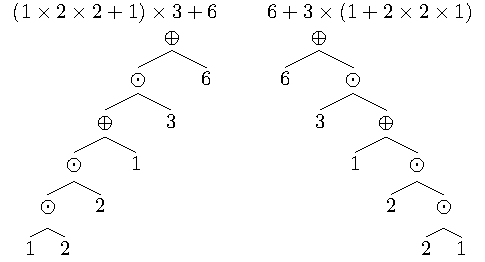
\includegraphics{images/03-example-expression-syntax-tree-left-right.pdf}}
\caption{right-expanded and left-expanded expressions}\label{fig:leftright}
\end{figure}

\begin{figure}[ht]
\centering
\resizebox{0.2\textheight}{!}{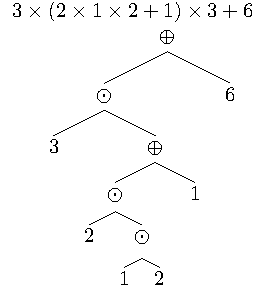
\includegraphics{images/04-example-expression-syntax-tree-combination}}
\caption{combinations of right-expanded and left-expanded expressions}\label{fig:combination}
\end{figure}

The evaluation order of an arithmetic expression is related to the topological order of its tree representation, but they are not the same.
The topological order of a tree is an ordering of nodes such that every node is visited before its parent\cite{Knuth1997TheAO}.
However, we are only interested in the ordering of branch nodes, as leaf nodes have already been evaluated and can be ignored.
Additionally, the topological order goes from parent to children, while the evaluation order goes from children to parent.

\begin{definition}
A threadlike expression is an arithmetic expression that all the left nodes in its tree representation are leaf nodes.
\end{definition}

So a threadlike expression is right-expanded and its evaluation order is unique.
One example of threadlike expressions is shown on the left side of Figure~\ref{fig:leftright}.

Threadlike expressions are significant here because they are analogous to the concept of paths in homotopy theory in geometry.
In a more general context, certain special types of threadlike expressions are also interesting:
for example, \emph{alternating threadlike expressions} are expressions in which the additional and multiplicative operators appear in an alternating manner.
In the field of computing, a hardware component called \emph{multiplier-accumulator} (MAC) unit has been implemented~\cite{Quinnell2007FloatingPointFM},
which is a special case of an alternating threadlike expression.
As a result, some numerical algorithms based on MAC units have been studied~\cite{Markstein2004SoftwareDA}.

\subsection{A scalar field and a mesh grid}\label{subsec:meshgrid}

Consider the upper half plane $\{\mathcal{H}: (x, y) | y > 0 \}$ equipped with an inner product and metrics defined as follows:

\[
\mathbf{a} \cdot \mathbf{b} = \begin{bmatrix} a_x & a_y \end{bmatrix} \begin{bmatrix} \frac{1}{y^2} & 0 \\ 0 & \frac{1}{y^2 \ln^2 2} \end{bmatrix} \begin{bmatrix} b_x \\ b_y \end{bmatrix}
\]

and

\[
ds^2 = \frac{1}{y^2} (dx^2 + \frac{dy^2}{\ln^2 2})
\]

We consider a scalar field satisfying

\begin{equation}
A = - \frac{x}{y}\label{eq:assignment}
\end{equation}

We call this field an \emph{assignment}.

Proper assignments allow us to establish a connection between paths in homotopy and threadlike arithmetic expressions,
and to incorporate function theory into the study of arithmetic expression geometry.

\begin{figure}[ht]
\centering
\resizebox{0.9\textwidth}{!}{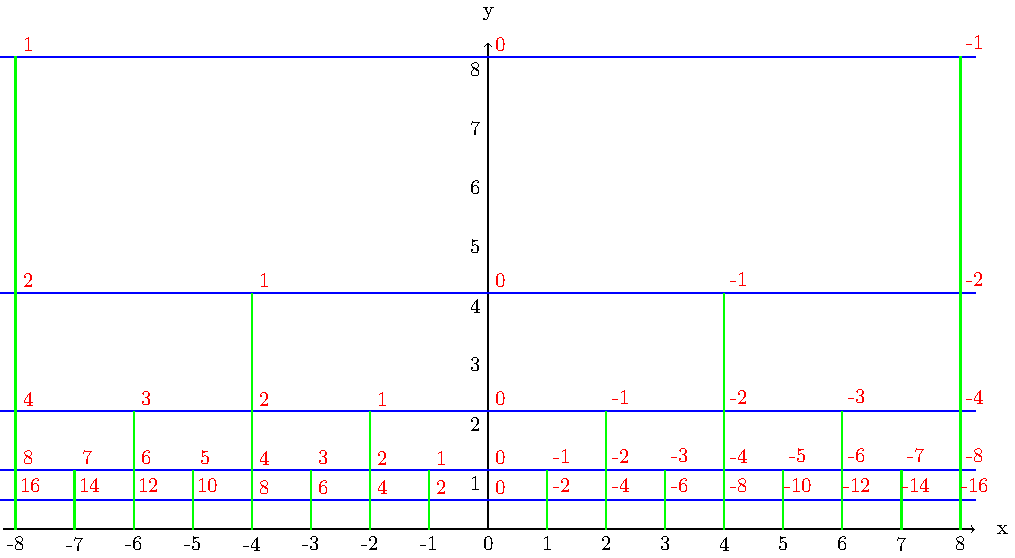
\includegraphics{images/01-grid-example-1.pdf}}
\caption{An addition-multiplication grid by generators with $\mu=1$ and $\lambda=\ln 2$}\label{fig:gridex0}
\end{figure}

We can draw a grid on the scalar field $A$ and underlying upper half plane $\mathcal{H}$ as shown in Figure~\ref{fig:gridex0}.
The blue lines encode a $+ 1$ relationship, the green lines encode a $\times 2$ relationship,
and they are line families that are perpendicular to each other.
The length of the line segments between two neighboring crossing points are unit length(calculations in lemma~\ref{lem:regular}).
The red value at the crossing points is the value of the scalar field $A$ at that point.
Based on the relationships encoded by the lines, we can encode threadlike arithmetic expressions,
which will be introduced in the subsection~\ref{subsec:encoding}.

The addition-multiplication grid is also scale-invariant under the transformation
\[
\begin{cases}
x' = \alpha x\\
y' = \alpha y
\end{cases}
\]

where $\alpha = 2^k , k \in \mathbb{Z}$.

We can image if we make the grid finer and finer, the grid will become a continuous space.
This leads to a rigorous treatment of arithmetic expressions as a geometric space in section~\ref{sec:topology}.

\subsection{Encoding threadlike expressions on the addition-multiplication grid}\label{subsec:encoding}

If we interpret the horizontal blue lines as $+ 1$ and the vertical green lines as $\times 2$ in Figure~\ref{fig:gridex0},
we can encode threadlike expressions on the addition-multiplication grid.
For example, in Figure~\ref{fig:encoding}
we encode $((((1 \times 4) - 1) \times 2) - 3)$ as the bold black lines.

\begin{figure}[ht]
\centering
\resizebox{0.9\textwidth}{!}{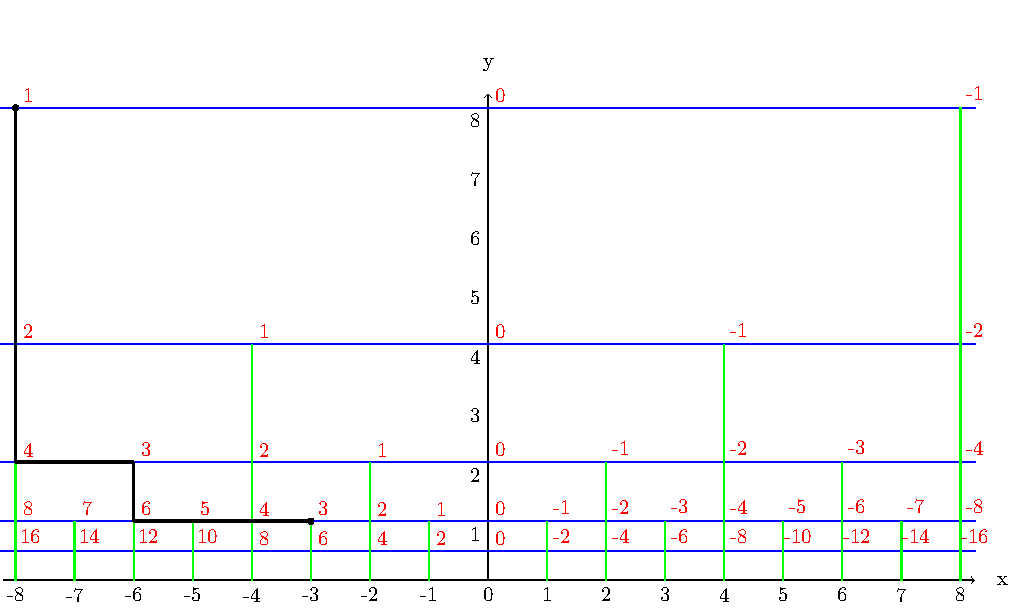
\includegraphics{images/05-example-expression-embedding}}
\caption{encoding threadlike expression}\label{fig:encoding}
\end{figure}

The zigzag lines in Figure~\ref{fig:encoding} can be divided into four parts:
\begin{itemize}
\item the vertical line from $1$ to $4$: encoded as multiplication by $4$
\item the horizontal line from $4$ to $3$: encoded as subtraction by $1$
\item the vertical line from $3$ to $6$: encoded as multiplication by $2$
\item the horizontal line from $6$ to $3$: encoded as subtraction by $3$
\end{itemize}

\subsection{From a scalar field to a space of threadlike expressions}\label{subsec:from-field-to-space}

As shown in Figure~\ref{fig:canonicalform}, we have the following paths and expressions:
\begin{itemize}
\item the black path: $((1 \times 8) - 5) = 3$
\item the purple path: $((1 - \frac{5}{8}) \times 8) = 3$
\item the brown path: $((((((1 - \frac{1}{8}) \times 2) - \frac{1}{2}) \times 2) - 1) \times 2) = 3$
\item the orange path: infinite many addition-multiplication terms accumulated together, a special kind of integration
\end{itemize}

\begin{figure}[ht]
\centering
\resizebox{0.9\textwidth}{!}{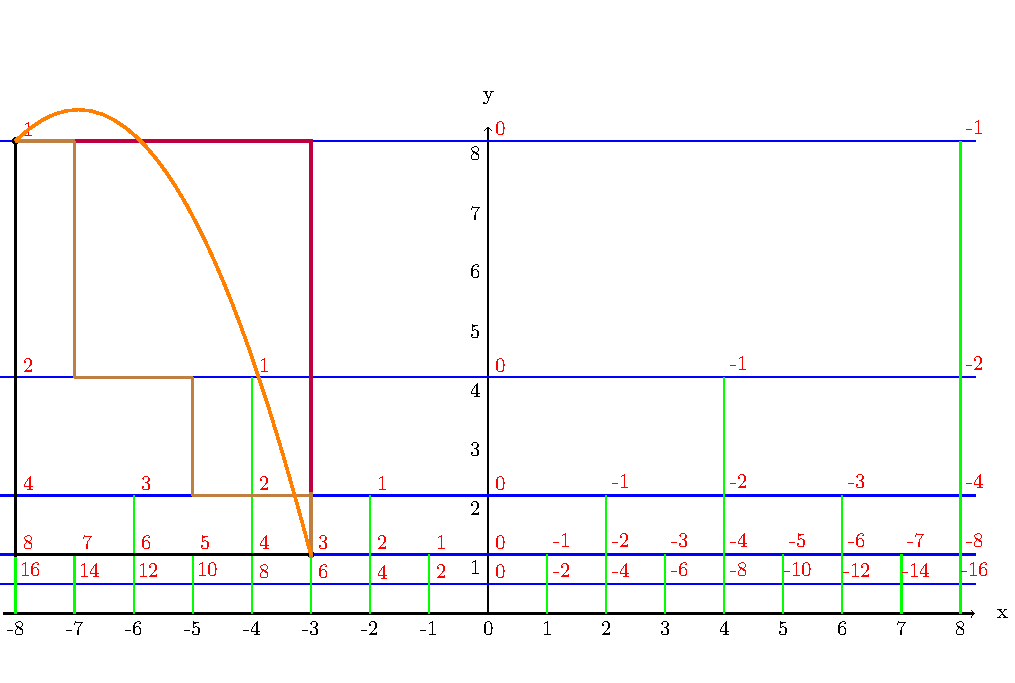
\includegraphics{images/06-example-canonical-form}}
\caption{different encodings and their canonical form}\label{fig:canonicalform}
\end{figure}

All of the paths in Figure~\ref{fig:canonicalform} have the same source $1$ and same target $3$.
We will discuss a canonical form for these paths.

It is easy to see that the expressions can be transformed into each other by using the multiplication distributive law and by combining and decomposing terms.

Conversion form brown path to black path
\begin{align}
3 & = ((((((1 - \frac{1}{8}) \times 2) - \frac{1}{2}) \times 2) - 1) \times 2) \\
& = 1 \times 8 -  \frac{1}{8} \times 8 - \frac{1}{2} \times 4 - 1 \times 2 \\
& = ((1 \times 8) - 5)
\end{align}

Conversion form brown path to purple path
\begin{align}
3 & = ((((((1 - \frac{1}{8}) \times 2) - \frac{1}{2}) \times 2) - 1) \times 2) \\
& = (1 - \frac{1}{8}) \times 8 - \frac{1}{2} \times 4 - 1 \times 2 \\
& = (1 - \frac{1}{8}) \times 8 - \frac{1}{4} \times 8 -  \frac{1}{4} \times 8 \\
& = (1 - \frac{1}{8} - \frac{1}{4} - \frac{1}{4}) \times 8 \\
& = ((1 - \frac{5}{8}) \times 8)
\end{align}

Therefore, we can define the black and purple paths in Figure~\ref{fig:canonicalform} as a pair of canonical paths,
which represent all threadlike expressions connecting the source $1$ and the target $3$.

Once we have such canonical paths, we can determine the canonical form of the whole space relative to an arbitrary source point $O$ and any other target point $P$.
This allows us to define the space as a space of threadlike expressions.

\subsection{Currying and path notation}\label{subsec:currying}

Currying is a basic technique in functional programming\cite{Reynolds1972DefinitionalIF},
which is used to transform a function with multiple arguments into a sequence of functions with one argument.
By currying a threadlike arithmetic expression, we can obtain a sequence of functions that operate on an operand, which is the leftmost leaf node.

We introduce the following notation for currying a threadlike arithmetic expression:
\begin{itemize}
    \item initial operand: the leftmost leaf node
    \item operator: $\oplus_y: x \mapsto x + y$
    \item operator: $\ominus_y: x \mapsto x - y$
    \item operator: $\otimes_y: x \mapsto x \cdot e^y$
    \item operator: $\oslash_y: x \mapsto x \cdot e^{-y}$
\end{itemize}

For example, the threadlike arithmetic expression $(((((1 \times 2) \times 2) + 1) \times 3) + 6)$ can be curried as

\[\oplus_6(\otimes_{\ln 3}(\oplus_1(\otimes_{\ln 2}(\otimes_{\ln 2}(1)))))\]

Suppose we have a series of operators $a_1, a_2, \cdots a_{n-1}, a_n$, we introduce a \emph{path notation}.

\[x a_1 a_2 \cdots a_{n-1} a_n \coloneqq a\_n( a_{n-1}( \cdots a_2( a_1(x) ) \cdots ) )\]

So, the above example can be written as

\[1 \otimes_{\ln 2} \otimes_{\ln 2} \oplus_1 \otimes_{\ln 3} \oplus_6 \]

If a path begins with a number, we refer to it as a \emph{bounded path}.
If it does not, we refer to it as a \emph{free path}, similar to the concept of vectors from the origin versus vectors at arbitrary points.
a bounded path results in a number, while a free path results in a function.

Now we will verify that the operators within a path are associative.

\begin{lemma}\label{lemma:associative}
    The operators within a path are associative, i.e. we have \[a [b c] = [a b] c\]
\end{lemma}

\begin{proof}
We use normal typeface to express the path notation, and bold typeface to express the function notation.

For a free path, follow the definition, we have
\[a [b c] = [b c](\mathbf{a}) = \mathbf{c}(\mathbf{b}(\mathbf{a}))\]
\[[a b] c = \mathbf{c}([a b]) = \mathbf{c}(\mathbf{b}(\mathbf{a}))\]

hence, we have
\[a [b c] = [a b] c\]
is hold for a free path.

For a bounded path, we have
\[x a [b c] = [b c](\mathbf{a}(x)) = \mathbf{c}(\mathbf{b}(\mathbf{a}(x)))\]
\[x [a b] c = \mathbf{c}([a b](x)) = \mathbf{c}(\mathbf{b}(\mathbf{a}(x)))\]

hence, we have
\[a [b c] = [a b] c\]
is hold for a bounded path.

\end{proof}

\begin{definition}\label{definition:concatenate}
    The concatenation of paths $p_1 \cdot p_2$ is defined as the composite of functions:
    \[p_1 \cdot p_2 \coloneqq p_2 \circ p_1 \]
\end{definition}

When a sequence of paths is concatenated, and only the first path can be bounded.
If the first path is bounded, the concatenated result is a bounded path.
Otherwise, the concatenated result is a free path.

\subsection{Alternating threadlike expressions}\label{subsec:alternating}

Now we can define alternating threadlike expressions, which were mentioned in Section~\ref{sec:expression}, using the path notion.

\begin{equation}\label{eq:alternative}
    \alpha = a_1 b_1 a_2 b_2 \cdots a_l b_l, a_i = \otimes_{\lambda_i}, b_i = \oplus_{\mu_i}, \lambda_i, \mu_i \in \mathbb{R}
\end{equation}

where $\bigoplus$ and $\bigotimes$ denote addition and multiplication, respectively,
and the expression is a zigzag of alternating addition and multiplication operations.
$\alpha$ is a free path, and we can bind a number to it.

Since $0$ is the identity element for addition and $1$ is the identity element for multiplication,
it is straightforward to see that any arithmetic expression can be converted into an alternating threadlike expression
by introducing more $0$ and $1$ into the original expression.
So alternating threadlike expression is a kind of canonical form.

We can derive a formula for perturbations in alternating threadlike expressions.

Let us define the left-to-right accumulated sum of $\lambda_i$ as $\check{\lambda}_i$, such that:
\begin{equation}
\check{\lambda}_i = \sum_{j=1}^i \lambda_j, \check{\lambda}_0 = 0\label{eq:accsumlr}
\end{equation}

Then we also have right-to-left accumulated sum of $\lambda_i$
\begin{equation}
\hat{\lambda}_i = \check{\lambda}_l - \check{\lambda}_{l - i}, \hat{\lambda}_0 = 0\label{eq:accsumrl}
\end{equation}

Expanding equation~\eqref{eq:alternative} using the distributive law and the above notion at point $\mu_0$, we obtain:
\begin{align}
\alpha(\mu_0) & = e^{\lambda_l}(\cdots (e^{\lambda_2} (e^{\lambda_1} \mu_0 + \mu_1) + \mu_2) \cdots) + \mu_l \\
& = e^{\hat{\lambda}_l} \mu_0 + e^{\hat{\lambda}_{l - 1}} \mu_1  + e^{\hat{\lambda}_{l - 2}} \mu_2 + \cdots + e^{\hat{\lambda}_1} \mu_{l - 1} + e^{\hat{\lambda}_0} \mu_l
\end{align}

Next, at the starting point $\mu_0$, we introduce a perturbation $\tilde{\mu}_0 = e^{\eta_0} \mu_0 + \epsilon_0$,
where $\eta_0$ and $\epsilon_0$ are the disturbance terms added by the summation and multiplication operations, respectively. Then, we have:
\begin{align}
\alpha(\tilde{\mu}_0) & = e^{\hat{\lambda}_l} (\tilde{\mu}_0) + e^{\hat{\lambda}_{l - 1}} \mu_1  + e^{\hat{\lambda}_{l - 2}} \mu_2 + \cdots + e^{\hat{\lambda}_1} \mu_{l - 1} + e^{\hat{\lambda}_0} \mu_l \\
& = \alpha(\mu_0) + e^{\hat{\lambda}_l} (\tilde{\mu}_0 - \mu_0)
\end{align}

As a result, purely from an arithmetic perspective, without the need for limits, we can derive the following meaningful ratio:
\begin{equation}
\frac{\alpha(\tilde{\mu}_0) - \alpha(\mu_0)}{\tilde{\mu}_0 - \mu_0} = e^{\hat{\lambda}_l} = e^{\check{\lambda}_l}\label{eq:ratio}
\end{equation}

Now we extend this relationship from the starting point $\mu_0$ to the entire process, we define the recursive formula

\[
w_i = e^{\lambda_i} w_{i-1} + \mu_i, w_0 = 0
\]

and then we have

\begin{equation}
\frac{\tilde{w}_i - w_i}{\tilde{\mu}_0 - \mu_0} = e^{\check{\lambda}_i}, i \in \{1, ..., l\}\label{eq:perturbation1}
\end{equation}

So, we have

\[
\tilde{w}_i - w_i = e^{\check{\lambda}_i} (\tilde{\mu}_0 - \mu_0)
\]

and hence

\begin{equation}
\tilde{w}_i - w_i = e^{\lambda_i}(\tilde{w}_{i - 1} - w_{i - 1})\label{eq:perturbation2}
\end{equation}

That means the perturbation along the path is controlled by the multiplication terms of $e^{\lambda_i}$.

\subsection{Generated structure, commutator and arithmetic torsion}\label{subsec:generated-structure}

In order to study mesh grids like the one described in subsection~\ref{subsec:meshgrid},
we need to investigate the algebraic structure of the threadlike arithmetic expressions that are generated.

For real number $\mathbb{R}$ and elements $\mu, \lambda \in \mathbb{R}$, we consider all the arithmetical expressions
that are freely generated from
\begin{itemize}
    \item initial operand: $0$
    \item operator: $\oplus_\mu: x \mapsto x + \mu$
    \item operator: $\ominus_\mu: x \mapsto x - \mu$
    \item operator: $\otimes_\lambda: x \mapsto x \cdot e^\lambda$
    \item operator: $\oslash_\lambda: x \mapsto x \cdot e^{- \lambda}$
\end{itemize}

We denote these expressions as $E(\mu, \lambda)$, where $\mu$ is the additional generator and $e^\lambda$ is the multiplicative generator.
In cases where the context is clear, we may omit $\mu$ and $\lambda$ from the index.
Our goal is not to study only a single $E(\mu, \lambda)$, but rather to use a family of $E(\mu, \lambda)$ to approach a continuous space.

Since $\oplus_\mu$ and $\ominus_\mu$ are mutually inverse operations, it follows that $\otimes_\lambda$ and $\oslash_\lambda$ are also mutually inverse. This means that $E(\mu, \lambda)$ forms a group.
An intriguing observation is that the commutator of this group is not equal to identity generally,
especially the commutator of the generators.

\begin{equation}
x \oplus_\mu \otimes_\lambda \ominus_\mu \oslash_\lambda - x = \mu(1 - e^{-\lambda})\label{eq:commutator1}
\end{equation}
\begin{equation}
x \otimes_\lambda \oplus_\mu \oslash_\lambda \ominus_\mu - x = - \mu(1 - e^{-\lambda})\label{eq:commutator2}
\end{equation}

Or equivlently, we define below error $\tau$:

\begin{equation}
\tau = x \otimes_\lambda \oplus_\mu - x \oplus_\mu \otimes_\lambda = \mu(1 - e^\lambda)\label{eq:torsion}
\end{equation}

These errors are constant, indicating a type of torsion in the generated group.
And torsion $\tau$ is specifically referred to as the arithmetic torsion.

We will reveal that $\tau$ is related to the curvature of the surface in later sections.

\subsection{Problems on equality, singularity, symmetries}\label{subsec:problems-on-equality-singularity-symmetries}

From the perspective of computer science, it is useful to consider different levels of equality within freely generated structures.
\begin{itemize}
\item Literal equality: the finest level of equality, judged by the string representation of the expression
\item Syntactical equality: equality under certain syntactical rules
\begin{itemize}
\item When inverse operators exist, it forms a group
\item When the commutative and distributive laws exist, it can be considered an algebra
\end{itemize}
\item Semantic equality: the coarsest level of equality, judged by the evaluation of the expression
\end{itemize}

Literal equality is the strictest level of equality, and two different threadlike expressions are considered equal only if their string representations are exactly the same.
This level of equality may be too strict, as it may not be compatible with the evaluation of the expression.
However, under literal equality, the generated structure is the most rich and provides the base textures that can be woven into a space.

Semantic equality is the least strict level of equality, and two different threadlike expressions are considered equal if they evaluate to the same number.
This level of equality provides the total symmetrical resources of the space.

We can think of literal equality as the bottom and semantic equality as the top of a lattice,
with syntactical equality being a compromise between the two extremes.

To end this introduction part of the paper, we present several problems and speculations that drives our research.
These important problems arise from distance between syntactical and semantic structures.

\emph{Foundational problem}: A careful reader may have noticed that the definition~\ref{def:arithmetic-expression} is based on rational numbers $\mathbb{Q}$.
Why can't we use real numbers $\mathbb{R}$ instead?
The answer is that syntactically valid expressions may not be semantically valid.
Dividing by zero can lead to invalid expressions, and the evaluation of the expression cannot be defined in this situation.
Therefore, in real numbers, an expression may be syntactically valid but semantically not valid,
and there is no algorithm that can decide whether an expression is semantically valid or not.
How can we bridge this gap and provide a continuous geometry space?
We will attempt to partially solve this problem in some special cases in section~\ref{sec:topology}.

\emph{Singular point problem}: We have a very strong intuition that semantically invalid expressions lead to singular points.
The way we discussed in complex analysis may be borrowed here: essential singularities and poles.

\emph{Symmetry and classification problem}: We conjecture that the equality lattice may not only play a role in the construction of a space, but also determine the symmetry of that space.
We can imagine that, at certain levels of the lattice, we weave syntactically generated substructures into points to form a space,
and the weaving process uses up some symmetrical resources, leaving the rest to form a symmetry on the space.
The structure within the total symmetry may provide us with a systematic way of constructing spaces, and allow us to classify spaces based on their symmetries.
